% \begin{minipage}[t]{0.55\textwidth}
%   \centering
%   \includegraphics[width=\linewidth]{sections/method/figures/kvcache_system4.png}
%   % \captionof{figure}{
%   % Left: AR decoding is memory-bound due to KV cache growth and sequential token generation.
%   % Middle: DLM generation is compute-bound because it computes over the full sequence at every step.
%   % Right: Our method caches and reuses KV projections for clean tokens and restricts computation to a fixed-size window.}
%   \captionof{figure}{
%   \zhanqiu{Change color for the figure}
%   Left: AR decoding is memory-bound due to sequential token generation.
%   Middle: DLM generation is compute-bound because it computes over the full length.
%   Right: Our method caches and reuses KV projections for clean tokens and restricts computation to a fixed-size window.}
% \label{fig:kvcache}
% \end{minipage}%
% \hfill
% \begin{minipage}[t]{0.42\textwidth}
%   \centering
%   \includegraphics[width=\linewidth]{figures/guided_unmasking.pdf}
%   \captionof{figure}{
%     \textbf{Placeholder for guided unmasking}
%   }
% \label{fig:pareto}
% \end{minipage}


% \begin{figure}[t!]
%     \centering
%     \includegraphics[width=0.9\linewidth]{sections/method/figures/FreeCache.png}
%     \caption{Proposed training-free block-wise caching strategy with diffusion language model.}
%     \label{fig:enter-label}
% \end{figure}

% % \begin{figure}[t!]
% \begin{figure}[H]
%     \centering
%     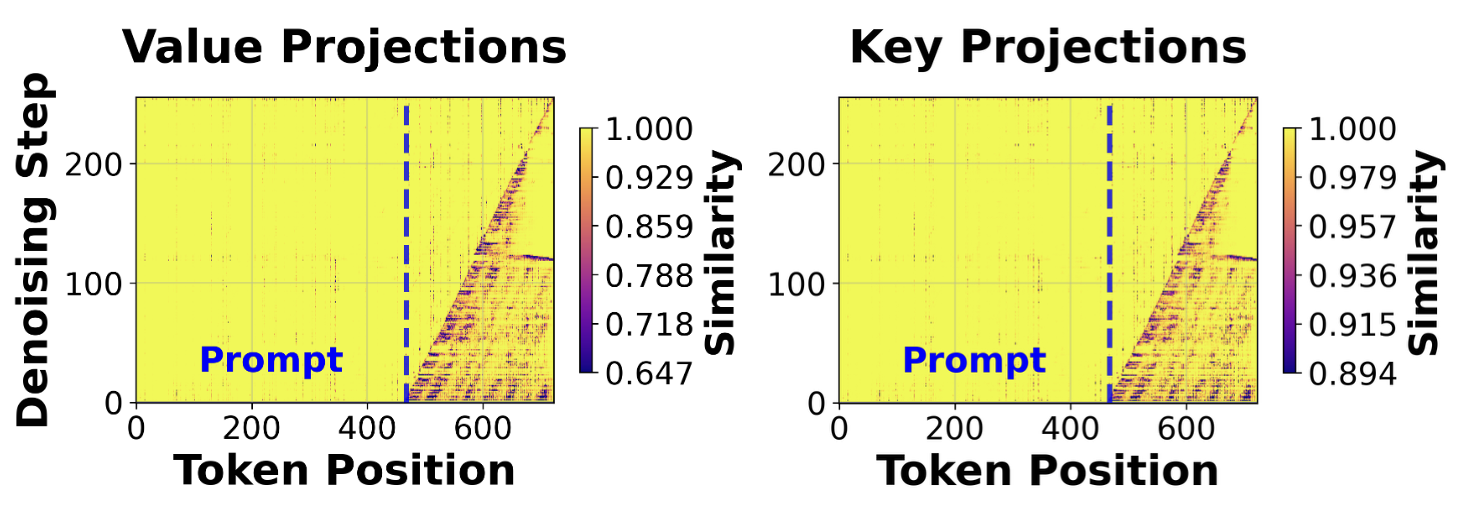
\includegraphics[width=1\linewidth]{sections/method/figures/kv_projections.png}
%     \caption{Rationale behind the proposed FreeCache: The variation of K and V projections of clean tokens is small throughout the subsequent diffusion steps. }
%     \label{fig:freecache_rationale}
% \end{figure}

\begin{table}[t!]
\caption{Latency and accuracy of the proposed FreeCache with different Diffusion Language Models. The proposed method achieves 4.42$\times$ and 6.32$\times$ speedup on Dream-7B-Instruct and LLaDA-8B-Instruct models.}
\label{tab:freecache_results}
\resizebox{\linewidth}{!}{\begin{tabular}{ccccc}
\toprule
\textbf{Models}                             & \textbf{Method}                & \textbf{GSM8K (8-shot) Accuracy (\%)} & \textbf{Raw Latency (s)} & \textbf{Speedup}       \\ \midrule
\multirow{2}{*}{Dream-7B-Instruct~\cite{dream2025}} & Baseline              & 79.68               & 48.05           & 1.0 $\times$  \\ \cmidrule{2-5} 
                                   & \textbf{FreeCache (This work)} & 77.40               & \textbf{10.87}           & \textbf{4.42}$\times$  \\ \midrule
\multirow{2}{*}{LLaDA-8B-Instruct~\cite{nie2025large}}          & Baseline              & 79.30               & 56.89           & 1.0 $\times$  \\ \cmidrule{2-5} 
                                   & \textbf{FreeCache (This work)} & 77.18               & \textbf{9.02}            & \textbf{6.32}$\times$ \\ \bottomrule
\end{tabular}}
\end{table}